\chapter{Analysis and Findings}
\label{ch:analysis}

\section{Overview}

This chapter reports results from the final, verified dataset: 900 LLM responses (300 profiles $\times$ 3 strategies), confirmed to contain zero duplicate profile--strategy pairs, with the zero-shot and few-shot strategies in the corrected reasoning-required format described in Section~3.4.2. Section~\ref{sec:rq1rq2} addresses Research Questions 1 and 2 (recommendation quality and the effect of prompting strategy); Section~\ref{sec:archetype} reports the per-archetype breakdown; Section~\ref{sec:factual} addresses Research Question 3 (factual correctness); Section~\ref{sec:explanation-consistency} reports on explanation quality and consistency (Research Questions 3 and 4).

\section{Recommendation Quality by Prompting Strategy}
\label{sec:rq1rq2}

Table~\ref{tab:overlap-summary} summarises the overlap score (proportion of the baseline's top-3 cards also present in the LLM's top three) and top-1 exact-match accuracy for each strategy, across all 300 profiles.

\begin{table}[htbp]
\centering
\caption{Recommendation-quality summary by prompting strategy (n=300 profiles per strategy)}
\label{tab:overlap-summary}
\begin{tabular}{lccccc}
\toprule
Strategy & Mean overlap & Median overlap & Std.\ dev. & Mean top-1 acc.\ & \% zero-overlap \\
\midrule
Zero-shot   & 0.687 & 0.667 & 0.258 & 0.307 & 6.0\% \\
Structured  & 0.517 & 0.333 & 0.299 & 0.077 & 10.7\% \\
Few-shot    & 0.539 & 0.667 & 0.324 & 0.023 & 18.7\% \\
\bottomrule
\end{tabular}
\end{table}

Contrary to expectations set by the wider few-shot-learning literature (Section~2.2), \textbf{zero-shot prompting produced the strongest recommendation-quality results on every measure}: the highest mean overlap with the baseline (0.687, against 0.517 for structured and 0.539 for few-shot), the highest top-1 exact-match accuracy by a wide margin (0.307, roughly four times the structured rate and thirteen times the few-shot rate), and the lowest proportion of profiles receiving zero overlapping recommendations (6.0\%, against 18.7\% for few-shot).

A Kruskal-Wallis test confirms this difference is statistically significant across the three strategies: $H = 60.70$, $p = 6.6 \times 10^{-14}$ (well below the $p < 0.05$ threshold). Pairwise paired Wilcoxon signed-rank tests, matched at the profile level (Table~\ref{tab:wilcoxon}), show that zero-shot significantly outperforms both structured ($W = 6996.0$, $p < 0.0001$) and few-shot ($W = 10097.5$, $p < 0.0001$), while the difference between structured and few-shot narrowly fails to reach significance at the conventional threshold ($W = 19809.0$, $p = 0.0588$).

\begin{table}[htbp]
\centering
\caption{Paired Wilcoxon signed-rank tests, per-profile mean overlap score}
\label{tab:wilcoxon}
\begin{tabular}{lccc}
\toprule
Comparison & $W$ & $p$-value & Significant ($p<0.05$) \\
\midrule
Zero-shot vs.\ Structured & 6996.0  & $<0.0001$ & Yes \\
Zero-shot vs.\ Few-shot   & 10097.5 & $<0.0001$ & Yes \\
Structured vs.\ Few-shot  & 19809.0 & 0.0588    & No \\
\bottomrule
\end{tabular}
\end{table}

Figure~\ref{fig:overlap-boxplot} shows the distribution of overlap scores by strategy, and Figure~\ref{fig:prompt-comparison} shows the combined per-strategy comparison generated by the analysis pipeline.

\begin{figure}[htbp]
\centering
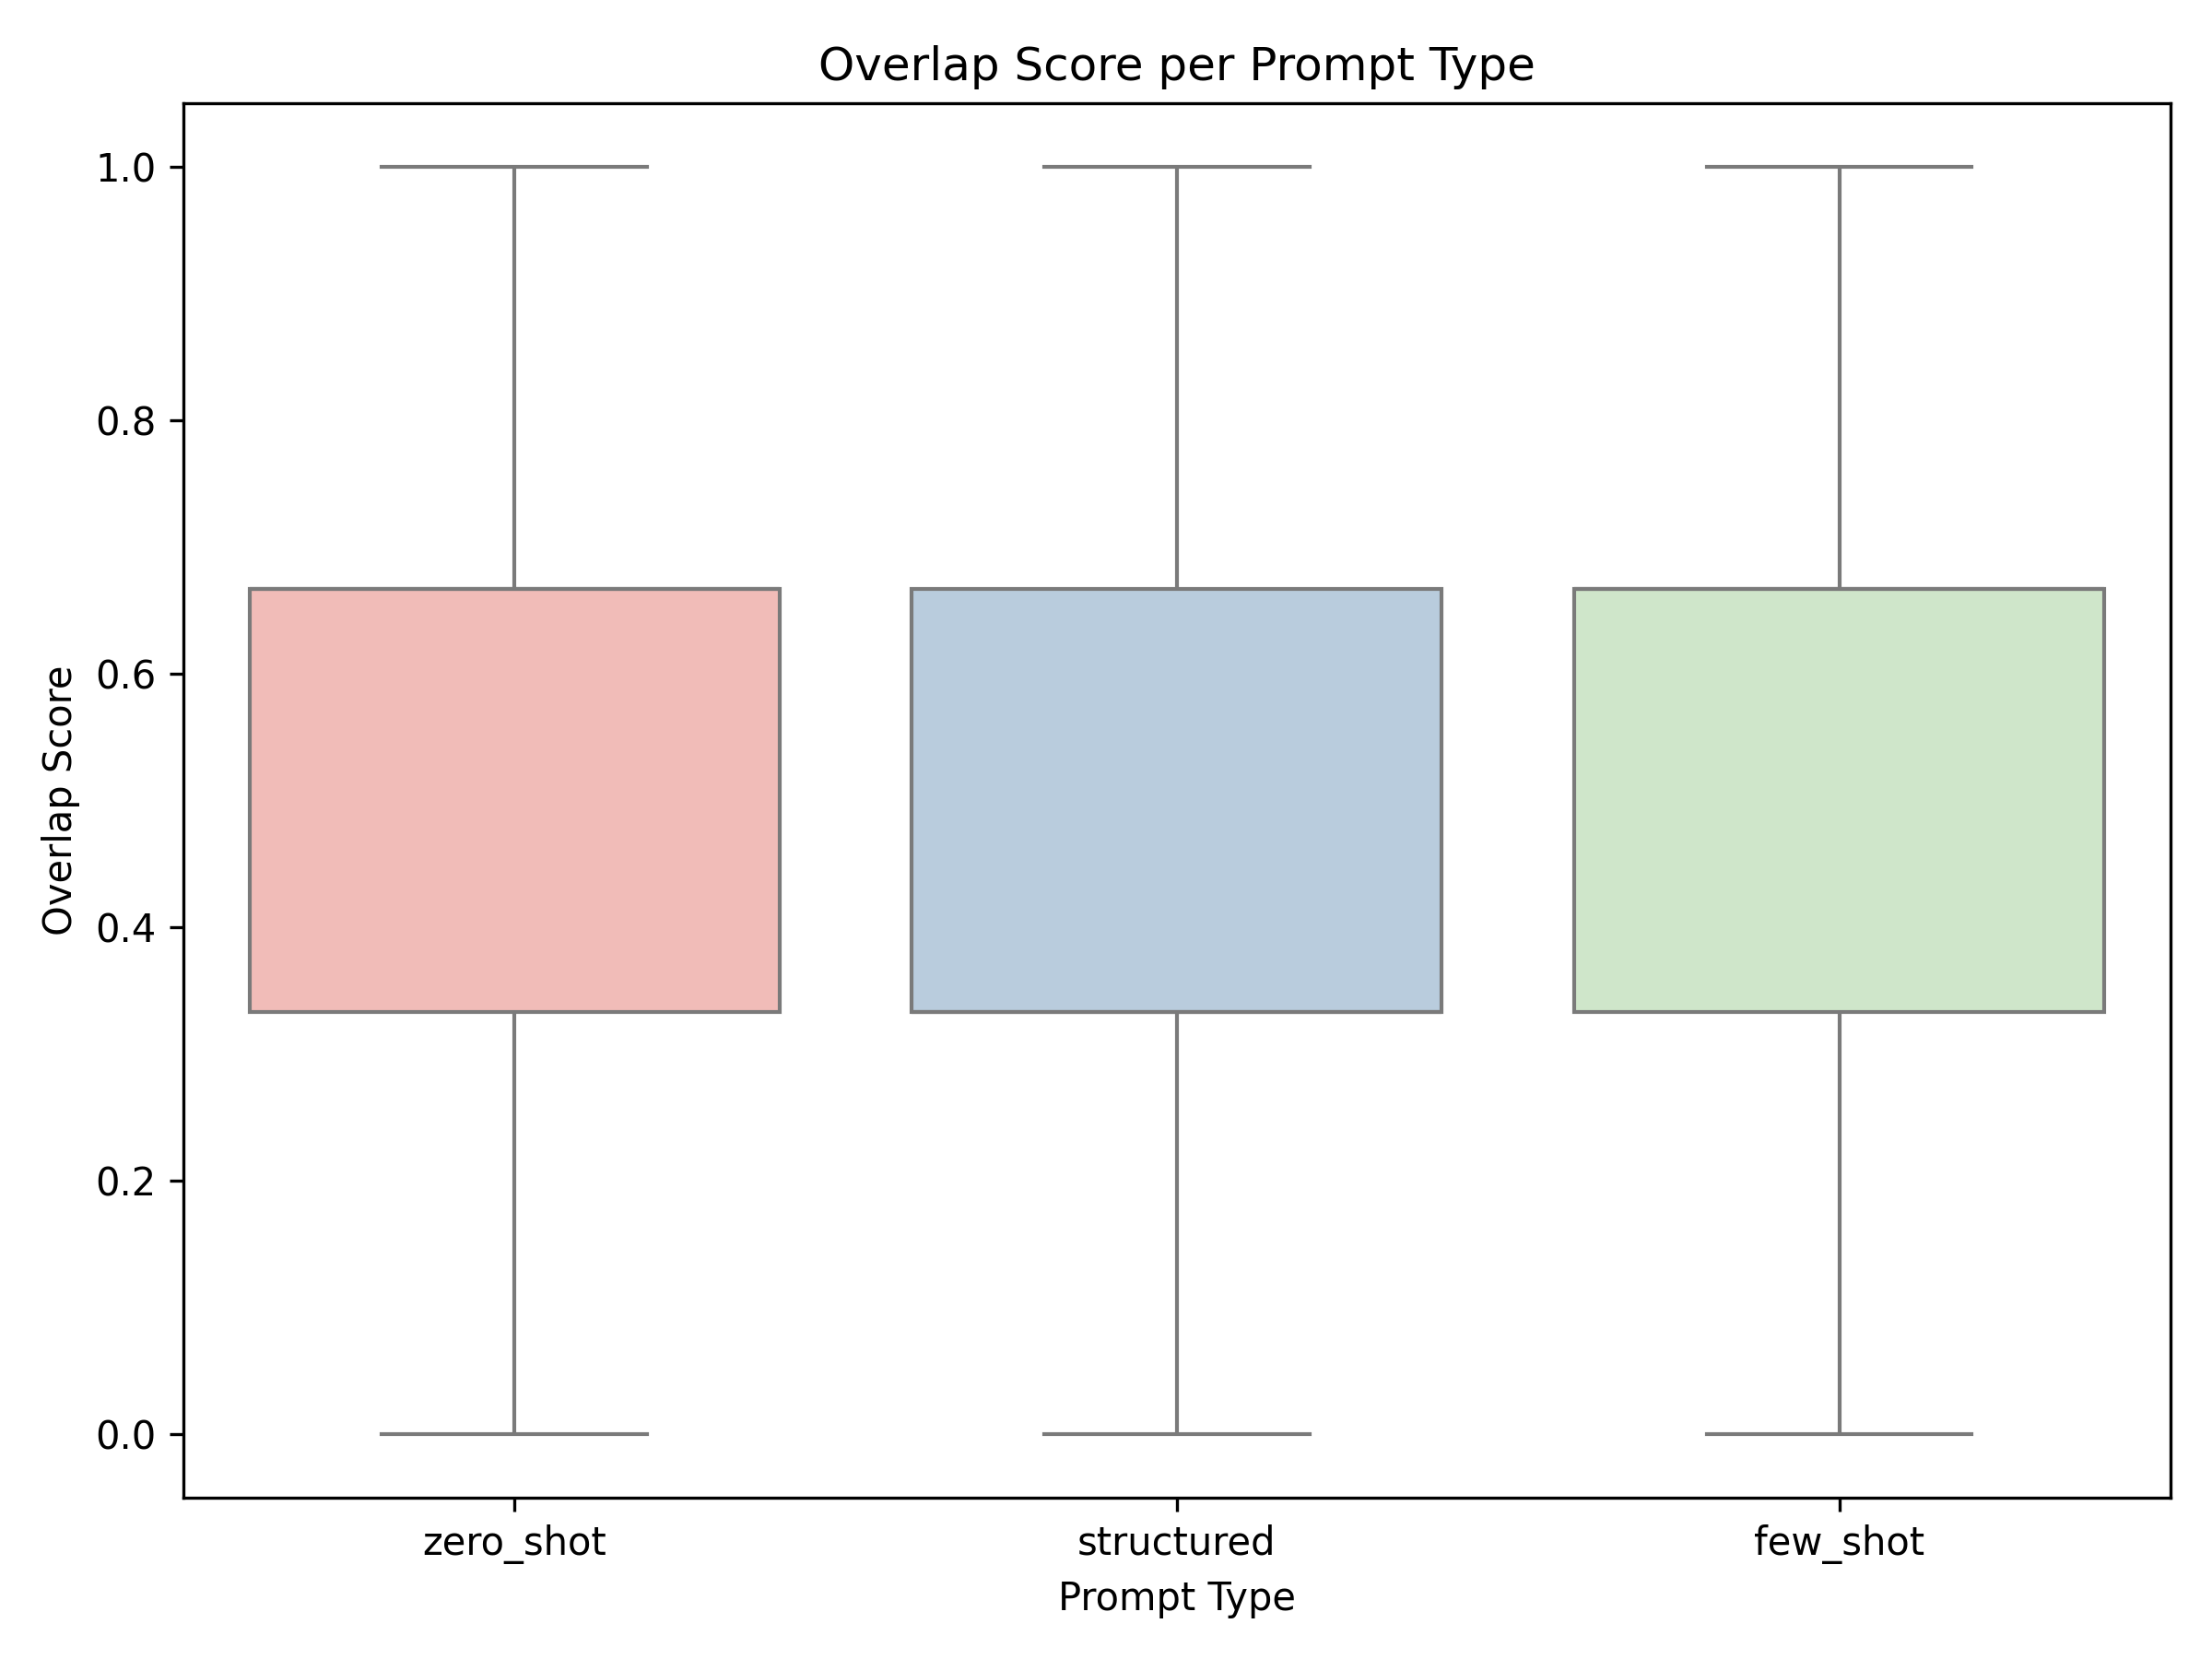
\includegraphics[width=0.75\textwidth]{results/overlap_boxplot.png}
\caption{Distribution of overlap scores by prompting strategy}
\label{fig:overlap-boxplot}
\end{figure}

\begin{figure}[htbp]
\centering
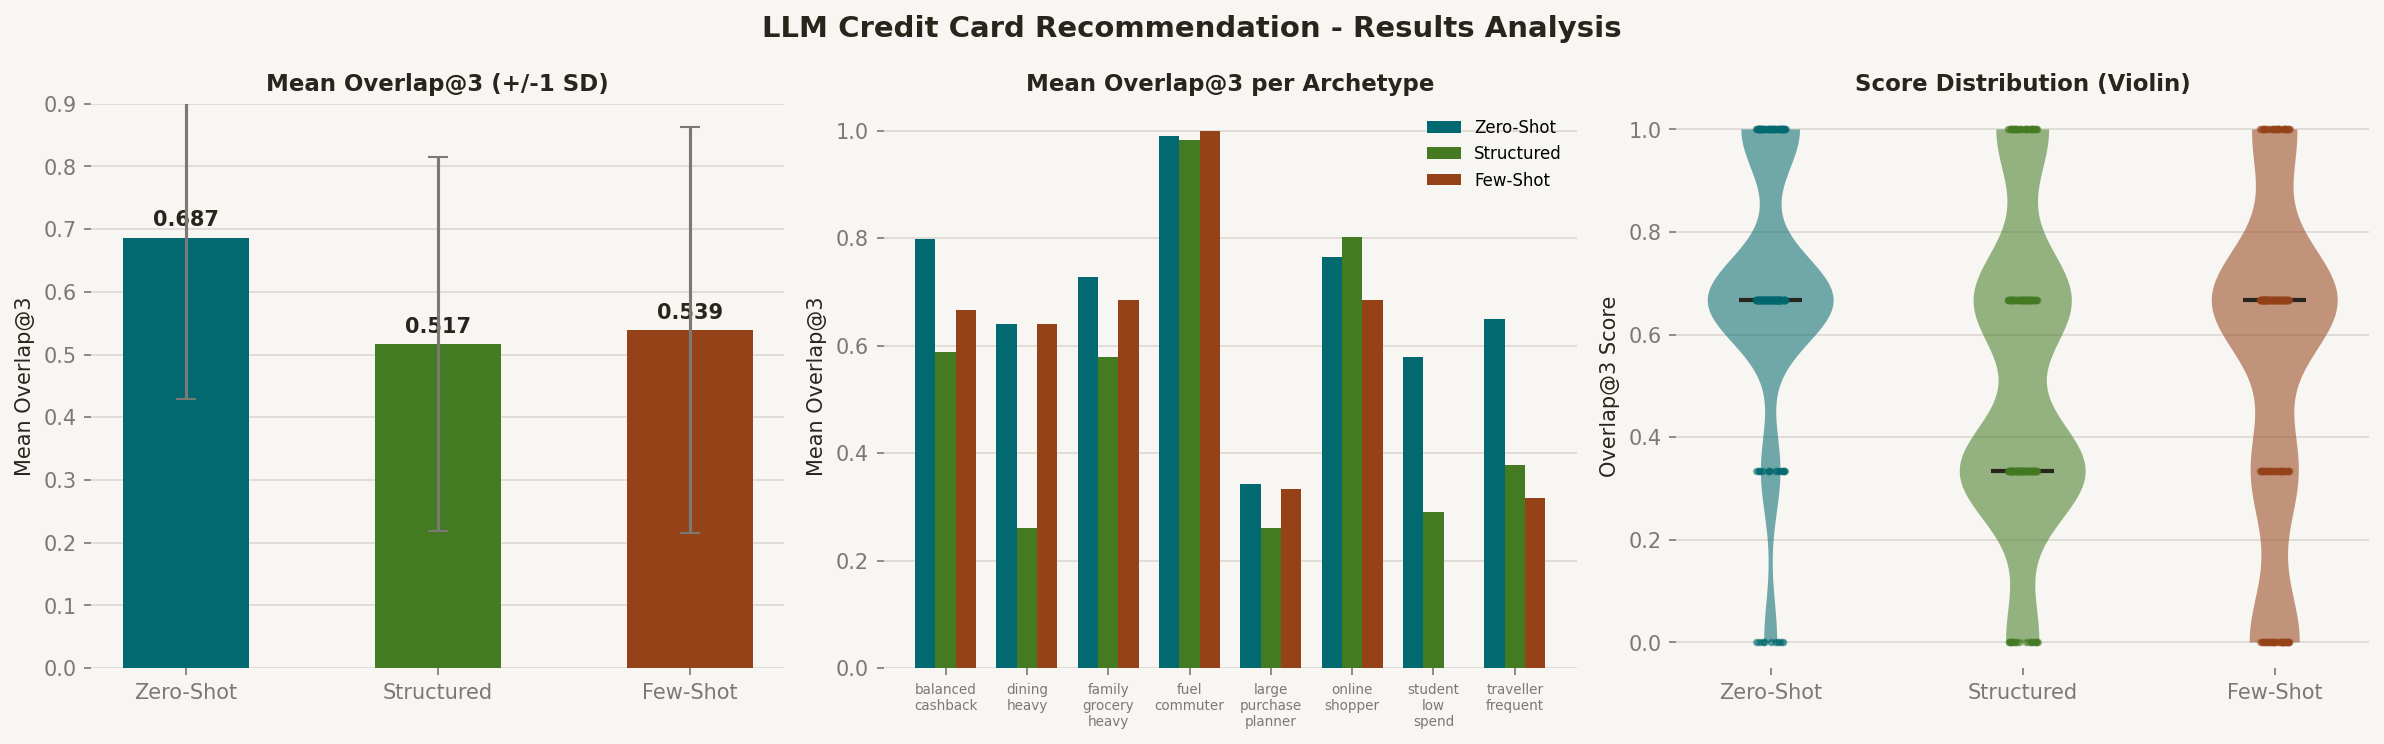
\includegraphics[width=0.85\textwidth]{results/figures/prompt_comparison.png}
\caption{Combined recommendation-quality comparison across strategies}
\label{fig:prompt-comparison}
\end{figure}

This result is discussed in relation to the prompt-engineering literature in Section~\ref{sec:discussion-rq}: it is a genuine, counter-to-expectation finding rather than a data artefact, and one plausible explanation --- that the additional instruction text and worked examples in the structured and few-shot conditions crowd out the model's attention on the profile's specific attributes, at only 8 billion parameters --- is explored further in Chapter~\ref{ch:discussion}.

\section{Per-Archetype Breakdown}
\label{sec:archetype}

Table~\ref{tab:archetype} reports mean overlap and top-1 accuracy separately for each of the eight consumer archetypes, to check whether the strategy effect found in Section~\ref{sec:rq1rq2} is uniform across consumer segments or archetype-dependent.

\begin{table}[htbp]
\centering
\caption{Mean overlap score and top-1 accuracy by archetype and strategy}
\label{tab:archetype}
\small
\begin{tabular}{lcccccc}
\toprule
& \multicolumn{3}{c}{Mean overlap} & \multicolumn{3}{c}{Mean top-1 accuracy} \\
Archetype & Zero-shot & Structured & Few-shot & Zero-shot & Structured & Few-shot \\
\midrule
Balanced cashback       & 0.798 & 0.588 & 0.667 & 0.368 & 0.000 & 0.000 \\
Dining-heavy            & 0.640 & 0.261 & 0.640 & 0.568 & 0.000 & 0.000 \\
Family, grocery-heavy   & 0.728 & 0.579 & 0.684 & 0.000 & 0.000 & 0.000 \\
Fuel commuter           & 0.991 & 0.982 & 1.000 & 0.081 & 0.081 & 0.000 \\
Large-purchase planner  & 0.342 & 0.261 & 0.333 & 0.054 & 0.027 & 0.162 \\
Online shopper          & 0.766 & 0.802 & 0.685 & 0.162 & 0.432 & 0.027 \\
Student, low-spend      & 0.579 & 0.289 & 0.000 & 0.237 & 0.000 & 0.000 \\
Frequent traveller      & 0.649 & 0.377 & 0.316 & 0.974 & 0.079 & 0.000 \\
\bottomrule
\end{tabular}
\end{table}

The zero-shot strategy's advantage is not uniform: it is dramatic for the \texttt{traveller\_frequent} archetype (97.4\% top-1 accuracy against 7.9\% for structured and 0\% for few-shot) and for \texttt{dining\_heavy} (56.8\% against 0\% for both other strategies), but the strategies converge closely for \texttt{fuel\_commuter}, where all three achieve near-perfect overlap (0.98--1.00) --- consistent with this archetype's spending profile mapping onto a small, easily-identified subset of the catalogue regardless of prompting approach. The \texttt{student\_low\_spend} archetype is the clearest failure case for few-shot prompting specifically, with a mean overlap of exactly 0.000, meaning the few-shot condition never once recommended a baseline top-3 card for this archetype across all 38 profiles; this is discussed further in Section~\ref{sec:discussion-rq}.

\section{Factual Correctness}
\label{sec:factual}

Table~\ref{tab:factual} summarises the deterministic factual-correctness check (Section~3.4.3) across all 900 responses.

\begin{table}[htbp]
\centering
\caption{Factual correctness by strategy}
\label{tab:factual}
\begin{tabular}{lcccccc}
\toprule
Strategy & Responses w/\ claims & Claims checked & Correct & Incorrect & Uncertain & \% error-free \\
\midrule
Zero-shot   & 170/300 & 1{,}800 & 864   & 771   & 165 & 55.0\% \\
Structured  & 300/300 & 1{,}715 & 1{,}247 & 346   & 122 & 73.7\% \\
Few-shot    & 232/300 & 3{,}150 & 1{,}021 & 2{,}117 & 12  & 24.0\% \\
\bottomrule
\end{tabular}
\end{table}

Structured prompting produces both the most consistently checkable responses (300/300 contain at least one checkable claim, against 170/300 for zero-shot and 232/300 for few-shot) and the highest accuracy rate on those claims (73.7\% of structured responses are entirely error-free, against 55.0\% for zero-shot). Few-shot prompting is a clear outlier in the opposite direction: despite generating the largest volume of checkable claims (3,150, roughly 1.8$\times$ structured's total), only 24.0\% of few-shot responses are entirely free of factual errors, and 2,117 of the 3,150 claims checked (67.2\%) were incorrect. This suggests the two worked examples in the few-shot prompt (Section~3.4.2) may lead the model to over-generate specific numeric claims about fees and reward rates by pattern-matching the examples' level of detail, without those specific figures being reliably grounded in the actual target card's data --- a hypothesis explored further in Chapter~\ref{ch:discussion}.

Combined with Section~\ref{sec:rq1rq2}, this produces a striking split rather than a single strategy dominating on every criterion: zero-shot leads on recommendation-baseline overlap, structured leads on factual reliability. Sections~\ref{sec:consistency-results} and~\ref{sec:explanation-consistency} add two further dimensions (consistency and explanation quality) to this picture, and --- as shown below --- the pattern becomes sharper still: no strategy leads on more than two of the four criteria, and few-shot in particular scores best on explanation quality while scoring worst on the two criteria that measure whether that explanation is actually accurate. This is precisely the kind of trade-off the four-criteria evaluation framework (Section~3.4.3) was designed to surface, and would not have been visible from recommendation-quality scoring alone.

\section{Consistency}
\label{sec:consistency-results}

Table~\ref{tab:consistency} reports the mean pairwise Jaccard similarity of the top-3 card set across three repeated runs, on the stratified 24-profile sample described in Section~3.4.4 (24 profiles $\times$ 3 strategies $\times$ 3 runs = 216 calls). A score of 1.0 means all three runs returned an identical top-3 set; 0.0 would mean no overlap at all between any pair of runs.

\begin{table}[htbp]
\centering
\caption{Consistency (mean pairwise Jaccard similarity across 3 runs) by strategy, n=24 profiles per strategy}
\label{tab:consistency}
\begin{tabular}{lcccc}
\toprule
Strategy & Mean & Std.\ dev.\ & Min & Max \\
\midrule
Zero-shot   & 0.826 & 0.200 & 0.500 & 1.000 \\
Few-shot    & 0.808 & 0.227 & 0.400 & 1.000 \\
Structured  & 0.776 & 0.184 & 0.467 & 1.000 \\
\bottomrule
\end{tabular}
\end{table}

All three strategies show reasonably high stability on average (0.78--0.83 on the 0--1 scale), and 13 of 24 zero-shot profiles and 13 of 24 few-shot profiles were perfectly stable (identical top-3 across all three runs), against 9 of 24 for structured. Numerically, zero-shot is the most stable strategy and structured the least, which is notable alongside Section~\ref{sec:factual}'s finding that structured is the \textit{most} factually reliable strategy --- a possible stability/reliability trade-off, discussed further in Chapter~\ref{ch:discussion}. However, a Kruskal-Wallis test across the three strategies on this metric is not statistically significant ($H = 0.78$, $p = 0.68$), so this difference should be read as a numerical trend on a modest stratified sample (24 profiles per strategy) rather than a confirmed effect --- unlike the recommendation-quality and factual-correctness results in Sections~\ref{sec:rq1rq2} and~\ref{sec:factual}, which are backed by the full 300-profile sample and are statistically significant.

The per-archetype pattern (not tabulated in full here; see \texttt{results/consistency\_scores.csv}) is uneven: \texttt{fuel\_commuter} and \texttt{traveller\_frequent} are highly stable across all three strategies (0.78--1.00), while \texttt{online\_shopper} and \texttt{dining\_heavy} show more run-to-run variation, particularly for few-shot (0.42 and 0.67 respectively) --- consistent with the pattern already seen in Section~\ref{sec:archetype}, where these strategies' performance is generally less uniform across archetypes.

\section{Explanation Quality}
\label{sec:explanation-consistency}

The explanation-quality criterion (LLM-as-judge, \texttt{src/llm\_judge.py}, Section~3.4.3) scores each response 1--3 on the clarity and grounding of its stated reasoning, using Llama 3.3 70B as judge --- a distinct, larger model than the one being evaluated, to reduce self-enhancement bias (Zheng et al., 2023). All 900 responses were judged. Table~\ref{tab:explanation-quality} summarises the results.

\begin{table}[htbp]
\centering
\caption{Explanation-quality scores (LLM-as-judge, 1--3 scale) by strategy, n=300 per strategy}
\label{tab:explanation-quality}
\begin{tabular}{lcccc}
\toprule
Strategy & Mean & Std.\ dev.\ & \% scored 3/3 & \% scored $\leq$1 \\
\midrule
Few-shot    & 2.907 & 0.291 & 90.7\% & 0.0\% \\
Zero-shot   & 2.730 & 0.459 & 73.7\% & 0.7\% \\
Structured  & 2.650 & 0.478 & 65.0\% & 0.0\% \\
\bottomrule
\end{tabular}
\end{table}

The result here is, on its own, the opposite of the recommendation-quality and factual-correctness findings: \textbf{few-shot prompting produces the highest-rated explanations} (mean 2.907/3, with 90.7\% of responses scoring the maximum), followed by zero-shot (2.730) and structured (2.650). A Kruskal-Wallis test confirms this is statistically significant ($H = 56.60$, $p = 5.1 \times 10^{-13}$), and all three pairwise Wilcoxon comparisons are also significant (zero-shot vs.\ structured $p = 0.016$; zero-shot vs.\ few-shot and structured vs.\ few-shot both $p < 0.0001$).

\subsection{Individual-Level Validity Check}
\label{sec:judge-validity}

The strategy-level pattern above raises an obvious question: does the judge's score for an individual response actually track that response's factual accuracy, or is the aggregate pattern a coincidence of strategy-level style differences? This is checked directly by merging the explanation-quality scores with the factual-correctness results (Section~\ref{sec:factual}) at the level of individual responses (n=702 responses with at least one checkable factual claim) and computing the correlation between judge score and factual accuracy for the same response. The result is a small but statistically significant \textit{negative} correlation between judge score and being factually error-free (point-biserial $r = -0.173$, $p < 0.0001$; mean judge score 2.801 for responses containing at least one factual error, against 2.642 for entirely error-free responses), and a small positive correlation between judge score and the raw \textit{number} of factual errors in a response (Spearman $\rho = 0.162$, $p < 0.0001$). In other words, the judge's scores do not merely fail to track factual accuracy at the individual-response level --- if anything, responses with more factual errors were rated very slightly \textit{higher} on average. This individual-level result reinforces, rather than merely coincides with, the strategy-level finding above, and is discussed as direct evidence for a verbosity/confidence bias in Chapter~\ref{ch:discussion}.

Read alongside Sections~\ref{sec:rq1rq2} and~\ref{sec:factual}, this produces the sharpest trade-off in the whole study: few-shot prompting writes the most highly-rated, clearest-\textit{sounding} explanations, while simultaneously being the least accurate against the baseline (mean overlap 0.539, Section~\ref{sec:rq1rq2}) and the least factually reliable (only 24.0\% of responses entirely error-free, Section~\ref{sec:factual}). In other words, on this task, a response reading as well-explained is not a reliable signal that it is either accurate or factually correct --- the worked examples in the few-shot prompt appear to teach the model to write in a more confident, detailed, well-structured style, without a corresponding improvement (indeed with a measurable decline) in whether that style is backed by correct facts. This is discussed further in Chapter~\ref{ch:discussion}.
